\section{Use case 1: Analysing blade grinder vibrations}
\SectionPage

\begin{frame}
    \frametitle{Goals}
    \vspace*{\fill}
    Improve blade-cutting machine line; has a high number of standstills and not ideal quality of the cut.
    \begin{figure}[ht]
        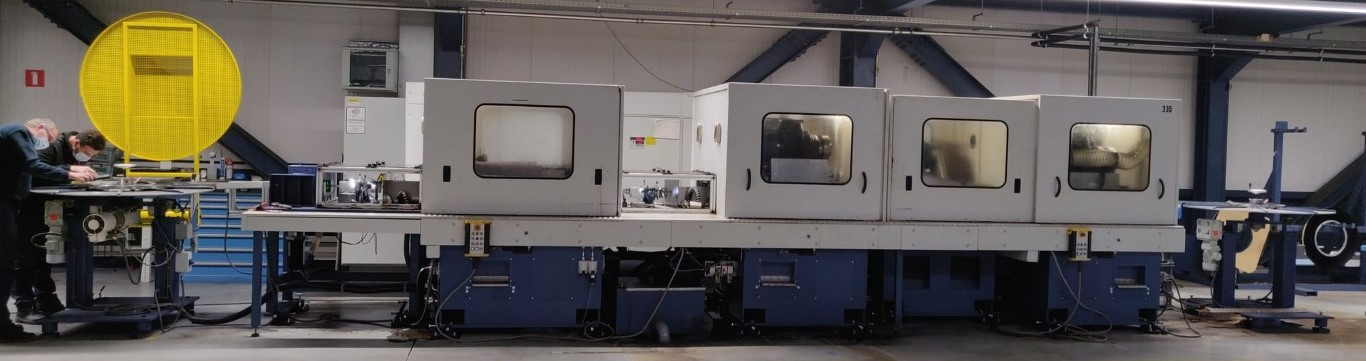
\includegraphics[width=0.95\linewidth]{stumabo/installation/line_photo.jpg}
        % \caption{Line overview: side view}
    \end{figure}
    \textbf{General goals}:
    \begin{itemize}
        \item Increase production quality
        \item Avoid unplanned standstill \& extend machines's life
        \item Identify the impact of the grindstones turning
        \item Find the root-cause of strong vibration
    \end{itemize}

    \vspace*{\fill}
\end{frame}

\begin{frame}
    \frametitle{Context}
    \begin{figure}[ht]
        \begin{subfigure}{\textwidth}
            \centering
            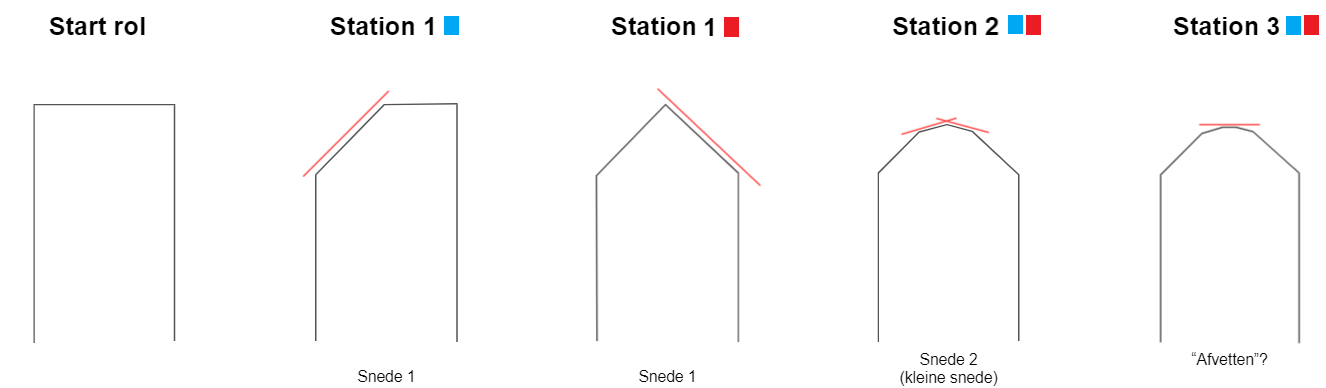
\includegraphics[width=0.65\textwidth]{stumabo/installation/blade_processing.png}
            % \caption{Blade evolution, a sketched overview of the cut by station}
        \end{subfigure}
        \begin{subfigure}{\textwidth}
            \centering
            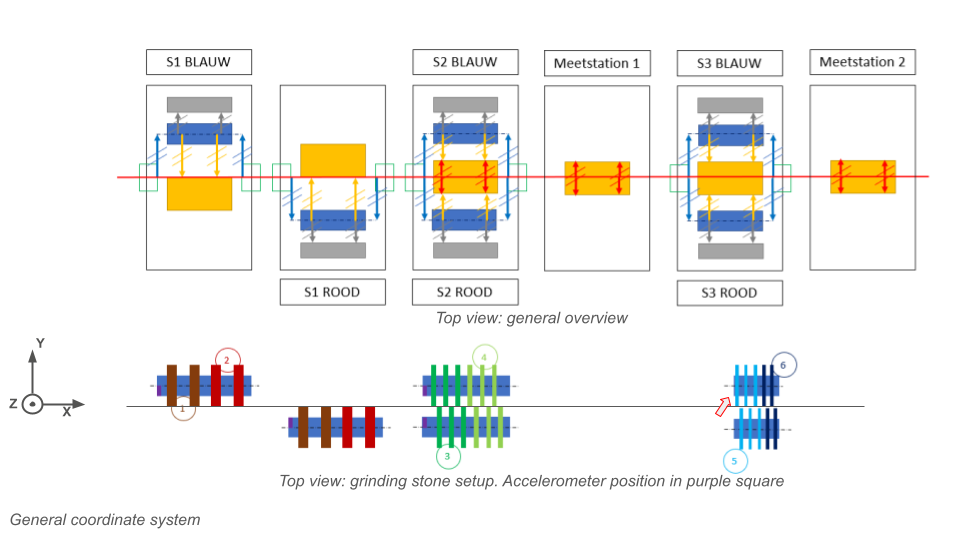
\includegraphics[width=0.67\textwidth]{stumabo/installation/general_cordinate_system.png}
            % \caption{Top view schematics}
        \end{subfigure}
        \caption{Blade evolution \& line top view; engineering schematics}
    \end{figure}
\end{frame}

% \subsection{4 Phases}
\begin{frame}
    \frametitle{4 Phases -- I}
    \vspace*{\fill}
    \begin{columns}[onlytextwidth, c]
        \begin{column}{.47\textwidth}
            \begin{exampleblock}{Hardware \& Data sources}
                \begin{itemize}
                    \item 3-dimension accelerometer
                    \item Mobile cabinet
                    \item Log file (operational data)
                \end{itemize}
            \end{exampleblock}
        \end{column}

        \begin{column}{.52\textwidth}
            \begin{figure}[ht]
                \begin{subfigure}{0.49\textwidth}
                    \centering
                    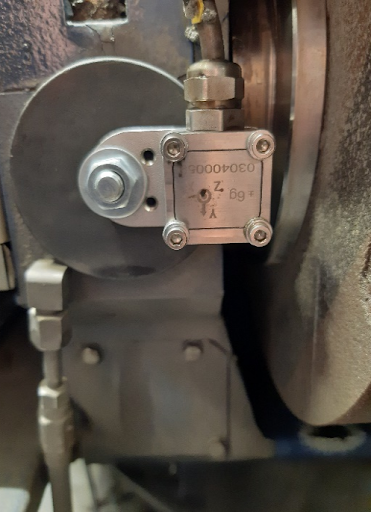
\includegraphics[height=\linewidth]{stumabo/installation/acc_station_1_blue.png}
                    \caption{Installation photo}
                \end{subfigure}
                \begin{subfigure}{0.49\textwidth}
                    \centering
                    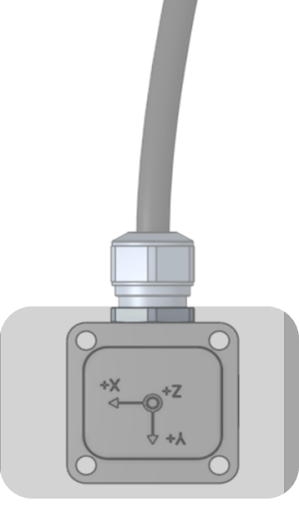
\includegraphics[height=\linewidth]{stumabo/installation/acc_render.png}
                    \caption{CAD render}
                \end{subfigure}
            \end{figure}
        \end{column}
    \end{columns}
    \vspace*{\fill}
\end{frame}

\begin{frame}
    \frametitle{4 Phases -- II}
    \vspace*{\fill}
    \begin{columns}[onlytextwidth, c]
        \begin{column}{.47\textwidth}
            \begin{exampleblock}{Installation}
                \begin{itemize}
                    \item \textcolor{red}{red} and \textcolor{blue}{blue} sides
                    \item Local $(x,y,z)$ for each sensor placement
                    \item Global $(X,Y,Z)$ for the entire production line
                    \item Sensor orientation and installation angle
                \end{itemize}
            \end{exampleblock}
        \end{column}
        \begin{column}{.52\textwidth}
            \begin{figure}
                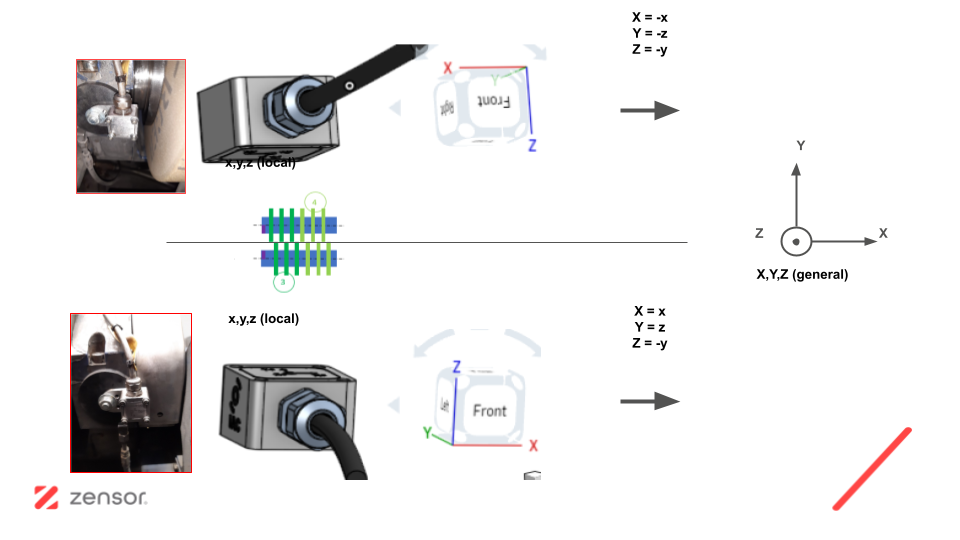
\includegraphics[width=\linewidth]{stumabo/installation/local_to_global.png}
                \caption{From local to general coordinate system}
            \end{figure}
        \end{column}
    \end{columns}
    \vspace*{\fill}
\end{frame}

\begin{frame}
    \frametitle{4 Phases -- III}
    \vspace*{\fill}
    \begin{columns}[onlytextwidth, c]
        \begin{column}{.47\textwidth}
            \begin{exampleblock}{Data Management}
                \begin{itemize}
                    \item Single data stream
                    \item  $ ACC_{x, y, z} \longrightarrow DB$
                    \item 60Hz to 1Hz /w Lambda
                \end{itemize}
            \end{exampleblock}
        \end{column}
        \begin{column}{.52\textwidth}
            \\
        \end{column}
    \end{columns}
    \begin{figure}[ht]
        \begin{subfigure}{0.495\textwidth}
            \centering
            \includegraphics[width=0.875\textwidth]{stumabo/analysis/60Hz-raw-vibration.pdf}
            \caption{60Hz raw vibration}
            \label{fig:stu_60Hz_raw}
        \end{subfigure}
        \begin{subfigure}{0.495\textwidth}
            \centering
            \includegraphics[width=0.875\textwidth]{stumabo/analysis/1Hz-raw-vibration.pdf}
            \caption{1Hz raw vibration}
            \label{fig:stu_1Hz_raw}
        \end{subfigure}
    \end{figure}
    \vspace*{\fill}
\end{frame}

\begin{frame}
    \frametitle{4 Phases -- IV}
    \vspace*{\fill}
    % Slide 1
    \begin{columns}[onlytextwidth, c]
        \begin{column}{.47\textwidth}
            \begin{exampleblock}{Analysis}
                \begin{enumerate}
                    \item \ac{EDA}
                    \item Isolate relevant blocks
                    \item Retrive ACC Data
                    \item Vector calculus: ${x, y, z} \rightarrow {X,Y,Z}$
                    \item \acl{RMS} (\acs{RMS})
                \end{enumerate}
            \end{exampleblock}
        \end{column}
        \begin{column}{.52\textwidth}
            \begin{figure}
                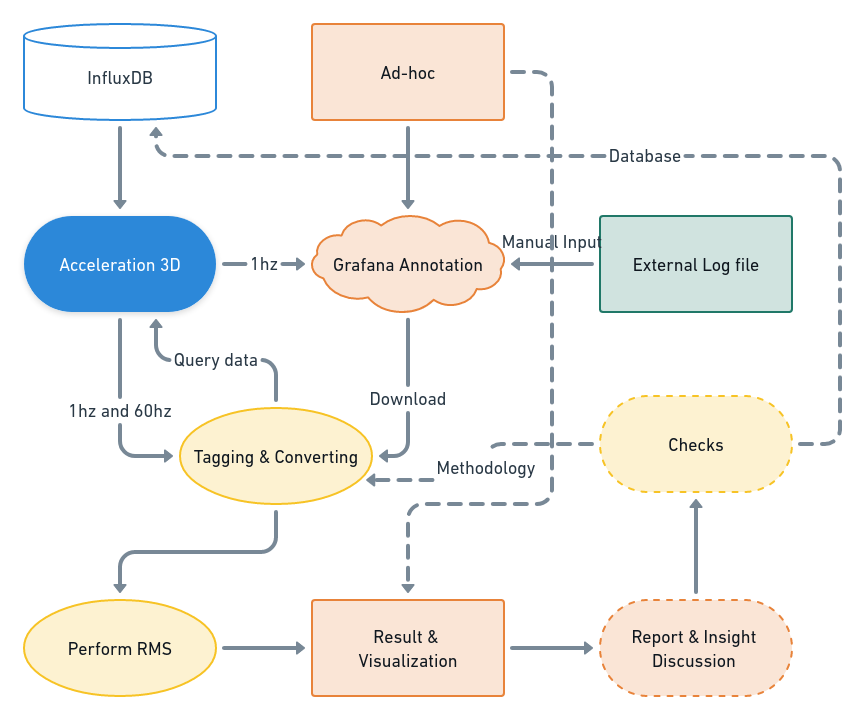
\includegraphics[width=\linewidth]{stumabo/analysis/analysis_flow.png}
                \caption{Steps involved during and after the analysis phase}
            \end{figure}
        \end{column}
    \end{columns}
    \vspace*{\fill}
\end{frame}

\begin{frame}
    \frametitle{Results}
    \vspace*{\fill}
    These plots were then discussed with a more experienced colleague, who had more domain knowledge.
    He also continued with the analysis.
    % decided not to discuss his insights, here
    % in this report, as they are not the result of my work but a more direct consequence.
    % Slide 2
    \begin{figure}[htp]
        \begin{subfigure}{.495\textwidth}
            \includegraphics[width=1.01\textwidth]{stumabo/analysis/1Hz-ad-hoc.pdf}
            \caption{1Hz RMS values}
            \label{fig:stu_1Hz_rms}
        \end{subfigure}
        \begin{subfigure}{.495\textwidth}
            \includegraphics[width=1.01\textwidth]{stumabo/analysis/60Hz-ad-hoc.pdf}
            \caption{60Hz RMS values}
            \label{fig:stu_60Hz_rms}
        \end{subfigure}
        % \begin{subfigure}{\textwidth}
        %     \includegraphics[width=\textwidth]{stumabo/analysis/1Hz-vs-60Hz.pdf}
        %     \caption{\texttt{1Hz} and \texttt{60Hz} RMS values}
        %     \label{fig:stu_1_vs_60}
        % \end{subfigure}
        \caption{RMS amplitude comparison \\between low and high frequency data}
        \label{fig:stu_3_rms}
    \end{figure}

    \vspace*{\fill}
\end{frame}

\begin{frame}
    \frametitle{Findings}
    \vspace*{\fill}

    The \textit{ad-hoc} analysis showed some insightful findings:
    \begin{enumerate}
        \item S1, \textcolor{blue}{blue} side, has higher vibration than expected
        \item S2 is the main source of vibration as we hoped it would be
        \item The cooling fluid, while drying, cause higher vibrations.
    \end{enumerate}

    \begin{alertblock}{Counter-intuitive result}
        Vibration amplitudes ($RMS_{X}$), along the blade going through the grinding stone stations, seemed \alert{more}
        prominent than in $Y$ direction, perpendicular to the blade direction.
    \end{alertblock}

    The stones turning would intuitively cause
    more vibrations perpendicular ($Y, Z$) to their rotating axe, not along $X$.\\
    After successfully double-checking the whole stack we can confirm that, indeed, $X$ and $Y$ are \structure{not} switched.
    \vspace*{\fill}
\end{frame}